\section{Modelos de función de base adaptativa}
\label{cap:adaptativa}

\subsection{Introducción}
\label{sec:intro_adap}

Esta sección se refiere a una familia general de modelos que llamaremos modelos de \textbf{función de base adaptativa}, que tienen la forma:
\begin{equation}
    f(x) = w_0 + \sum^K_{k=1} w_k \phi_k(x) \,. 
\end{equation}
A la función $\phi_k(x)$ se le dice la $m$-ésima función de base, la cual variará en función de los datos. Esta familia general de modelos incluye los modelos a estudiar en está sección: árboles, bosques, modelos basados en bagging y boosting, como también las redes neuronales y las sumas generales de modelos.


\subsection{Árboles}
\label{sec:arbol}

\subsubsection{Motivación con caso regresión}

Antes de definir árboles de manera formal, construiremos una intuición para el caso de regresión. Consideremos una función se una variable. Una idea, de aproximar tal función es hacer una interpolación usando funciones constantes. Una primera idea puede ser aproximar la función entera simplemente por su media.

\begin{figure}[h]
	\centering
	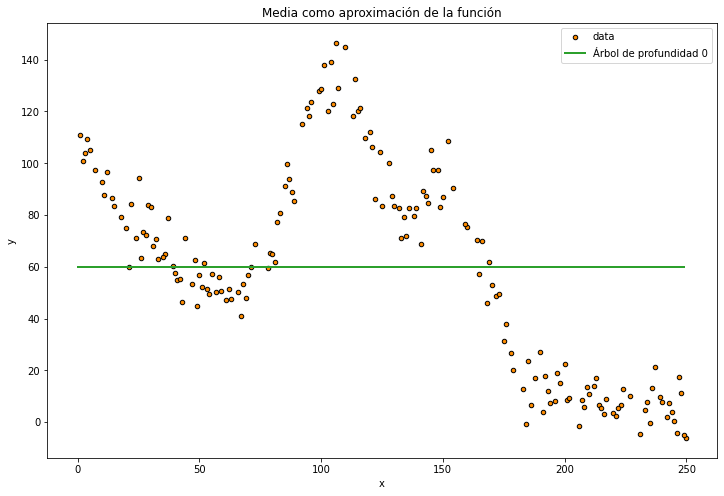
\includegraphics[width=0.5\textwidth, height=4.5cm]{img/capN_arbol_trivial.png}\\
	\caption{Aproximación de una función usando su media (árbol trivial no ajustado).}
\end{figure}

Otra manera, más bien voraz, de enfrentar el problema es realizar la interpolación con todos los puntos. Esto resultará con seguridad en un sobreajuste de los datos.

\begin{figure}[h]
	\centering
	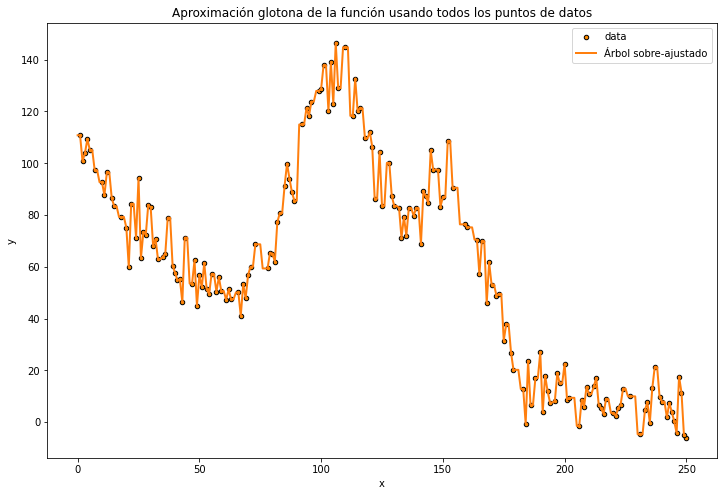
\includegraphics[width=0.5\textwidth, height=4.5cm]{img/capN_sobreajuste_arbol.png}\\
	\caption{Aproximación de una función usando todos los puntos de entrenamiento (árbol sobreajustado).}
\end{figure}

Una manera más inteligente consiste en agrupar ciertos puntos y hacer una interpolación usando la media de estos. El desafío es encontrar una partición conveniente del dominio de los datos de modo que al predecir un punto de nuestra función, tomar la media de los datos de entrenamiento para el subconjunto correspondiente resulte en una buena aproximación.

\begin{figure}[h]
	\centering
	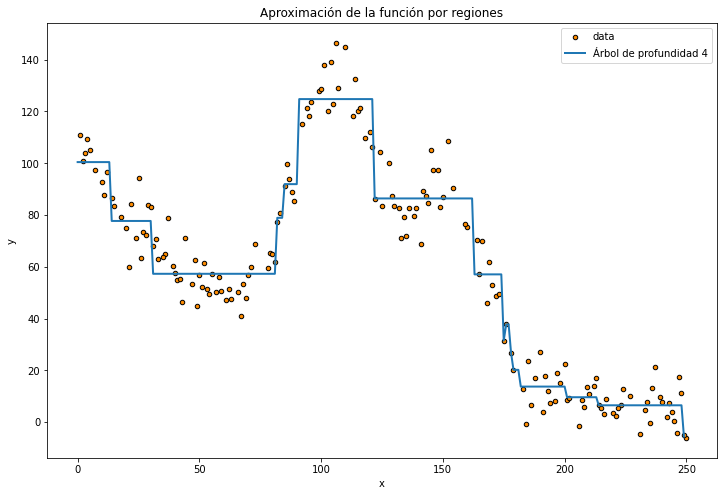
\includegraphics[width=0.5\textwidth, height=4.5cm]{img/capN_buen_arbol.png}\\
	\caption{Aproximación de una función con un árbol de profundidad adecuada.}
\end{figure}


\subsubsection{Algoritmo \textit{CART}}

Los árboles (de regresión) corresponden a ejecutar lo anterior de manera recursiva. Primero, necesitamos una algún criterio que nos indique si realizar un corte vale o no la pena. Para esto podemos definir el costo para un conjunto $D$ de datos como sigue:

\begin{equation}
    cost(D) = \sum_{i \in D} (y_i - \bar y)^2 \,,
\end{equation}

con $\bar y = \frac{1}{|D|} \sum_{i \in D} y_i $. Notemos como este costo es proporcional a la varianza empírica del conjunto D, con lo cual pedir bajo costo en los grupos de una partición se traduce en pedir que los datos estén cercanos a la media de tal subconjunto. Con esto podemos armar un algoritmo de base recursivo que genere un árbol de regresión.


\begin{algorithm}[H]
  \caption{Ajuste de árboles (CART)
    \label{alg:CART}}
  \begin{algorithmic}[1]
    \Function{ajusteArbol}{$nodo, D, profundidad$}
      \State $j^*, t^* = \arg\min_{j \in \{1,\dots,m\}, t \in \Gamma_j} \left[ cost(D_L(j,t)) + cost(D_R(j,t)) \right]$

        $D_L(j,t) = \{(x^{(i)}, y^{(i)}) : x_j^{(i)} \leq t \}$, $D_R(j,t) = \{(x^{(i)}, y^{(i)}) : x_j^{(i)} < t \}$
      
      \If{criterio\_de\_parada($costo, profundidad, D_I, D_D$)}:
        \Return{nodo}
      \Else
        \State $nodo$.izquierda = ajusteArbol($nodo, D_I, profundidad + 1$)
        \State $nodo$.derecha = ajusteArbol($nodo, D_R, profundidad + 1$)
        \Return{nodo}
    \EndFunction
  \end{algorithmic}
\end{algorithm}

Nótese que esto no necesariamente encontrará el árbol binario óptimo. Se prefiere este método voraz pues ajustar un árbol binario óptimo es un problema NP completo. En particular notemos como vamos separando coordenada por coordenada, lo cual nos hace ganar en interpretabilidad. Por otro lado, el 
 criterio de parada lo discutiremos más adelante.

Siguiendo el algoritmo anterior obtendremos una partición. Podemos enumerar los nodos de 1 hasta K. Con lo cual podemos recuperar la forma de base adaptativa:

\begin{equation}
    f(x) = \mathbb{E}[y | x] = \sum^K_{k=1} w_k \phi_k(x) \,,
\end{equation}

con $\phi_k(x) = \mathbf{1}_{D_k}(x)$ y $w_k = \frac{1}{|D_k|} \sum_{x^{(i) \in D_k}} y^{(i)}$. Como se señaló en la intuición, escogeremos la media de los datos en el subconjunto como predicción. Esto se justifica pues aquel valor es el que minimiza el error cuadrático. Podríamos también aprender un modelo simple (por ejemplo un regresor de mínimos cuadrados) de manera local en cada partición, sin embargo como hemos escogido la partición de manera que minimice la varianza, es razonable pensar que la media será una aproximación suficientemente buena.


\subsubsection{Criterios de corte para clasificación}

En el algoritmo CART hicimos uso de la función costo, que nos mostraba cuánto variaban los miembros de un intervalo respecto de la media. Podemos generalizar este mismo principio para clasificación, donde intentaremos caracterizar la impureza de etiquetas para un conjunto de manera adecuada. Primero tomemos el vector de probabilidades de pertenencia a una clase, condicionado a estar en un nodo. Sea $\mathcal{C}$ el conjunto de clases,

\begin{equation}
    \hat \pi_c (D) = \frac{1}{|D|} \sum_{x^{(i) \in D}} \mathbf{1}_{y=c}(y^{(i)}) \hspace{1cm} \, \forall c \in \mathcal{C} \,.
\end{equation}

Usando esto, para predecir la probabilidad de que un punto pertenezca a cada clase estará dado por el vector de fracciones empírica $\hat \pi$ correspondiente al nodo al cual pertenezca el dato en cuestión. Usemos este mismo vector para definir los criterios de impureza por nodo (ignoraremos la dependencia de D en el vector de probabilidades para simplificar la notación).

\begin{itemize}
    \item \textbf{Tasa de error} \\
    Sea $\hat y = \arg\max_{c \in \mathcal{C}} \hat \pi_c$ la clase más probable. El error estará dado por
    \begin{equation}
        cost(D) = \frac{1}{|D|} \sum_{x^{(i) \in D}} \mathbf{1}_{y = \hat \y}(y^{(i)}) = 1 - \hat \pi_{\hat y}
    \end{equation}
    El problema de este criterio es su poca sensibilidad a cambios en el vector de probabilidad. Los siguientes dos criterios mejoran esta situación.

    \item \textbf{Gini} \\
    Corresponde a la tasa de error esperado:
    \begin{equation}
        cost(D) = \sum_{c \in \mathcal{C}} \hat \pi_c (1 - \hat \pi_c) = 1 - \sum_{c \in \mathcal{C}} \hat \pi_c^2
    \end{equation}

    \item \textbf{Entropía} \\
    También llamada log-pérdida y muchas veces denotada por $H(\hat \pi)$, esta métrica está dada por:
    \begin{equation}
        cost(D) = - \sum_{c \in \mathcal{C}} \hat \pi_c log(\hat \pi_c) \,.
    \end{equation}
    Esta elección de perdida tiene justificación en la Teoría de la Información. En particular, su uso como criterio de corte equivale a la minimización de la entropía cruzada.
\end{itemize}

% En la figura se grafican los costos en función de la probabilidad de una clase en el caso clasificación binaria. 
Consideremos el ejemplo de clasificación binaria.  % TO DO: agregar imagen, descomentar linea anterior y borrar esta
Notemos que para las tres el máximo está cuando tenemos 50/50 de datos para cada clase en el nodo en cuestión, que es justamente el caso de mayor heterogeneidad de los datos. Por el contrario, los valores son cero cuando el conjunto tiene miembros de una sola clase. La sensibilidad antes mencionada se desprende de esto. En el caso de clases impuras, el error de clasificación está siempre por debajo de los otros criterios, que castigan más fuertemente la impureza.

% insertar figura


\subsubsection{Evitar sobreajuste: detención temprana y poda}

Una primera estrategia para evitar el sobreajuste del árbol es la \textbf{detención temprana}, i.e., evitar parar que se siga particionando el espacio. A continuación mencionaremos unos de los varios criterios, que se aplican como un criterio a verificar antes de seguir partiendo en el algoritmo \ref{alg:CART} (CART):

\begin{itemize}
    \item \underline{Máxima profundidad}:
    se puede imponer una profundidad máxima, de modo que una vez alcanzada esta no se separe más el nodo en cuestión.

    \item \underline{Número mínimo en nodo}: si un nodo contiene muy pocos datos entonces partirlo puede resultar en nodos con muy pocos datos (a este fenómeno se le llama fragmentación de datos). Podemos considerar o bien un entero o bien un porcentaje mínimo de los datos totales.

    \item \underline{Mínima reducción de costos}: Dados lados izquierdos y derechos de un corte, consideremos la reducción en costo como:
    \begin{equation}
        \Delta = cost(D) - \left[ \frac{|D_L|}{|D|} cost(D_L) + \frac{|D_R|}{|D|} cost(D_R) \right]
    \end{equation}
    Esta métrica de reducción de costos normalizada nos permite definir un criterio de parada donde no cortaremos el nodo si los nodos resultantes no inducen una reducción significativa. 
\end{itemize}

Los criterios anteriores inducen hiperparámetros que pueden ser
escogidos en una búsqueda de grilla.

La \textbf{poda} es otra estrategia para evitar el sobreajuste y disminuir la complejidad del árbol. Esta consiste en ajustar un árbol uno (posiblemente con criterios de parada anteriormente expuestos) y luego podarlo, que corresponde a elegir un sub-árbol (i.e., “podar” nodos). El conjunto de todos los subárboles de un árbol de decisión es potencialmente muy elevado. Es por esto que se elegirá un conjunto adecuado de subárboles, de modo que sea razonable comparar su rendimiento para elegir la mejor opción.

Primero consideraremos una métrica $R(T)$ que nos de una noción de costo para un árbol $T$. Típicamente se usará la suma de las tasas de errores (definidas anteriormente para clasificación y regresión) sumadas para cada hoja. Consideremos que el tamaño de un árbol $T$ es su número de hojas y denotemos aquello por $|T|$. Lo anterior nos permite definir una métrica que incorpora tanto el error como el tamaño de un árbol:

\begin{equation}
    R_\alpha (T) = R(T) + \alpha |T|
\end{equation}

Esta expresión se puede interpretar como agregar una penalización por complejidad si pensamos $\alpha$ como costo en complejidad de un nodo terminal. Notemos que a medida que se aumenta $\alpha$ más estaremos prefiriendo un árbol con menos hojas, por ende la métrica es sensible a tal hiperparámetro. Usaremos este hecho para construir un algoritmo que seleccione árboles adecuados de los cuales seleccionar el mejor, donde la idea se resume a continuación:

Dado el árbol original $T_0$, el objetivo será construir una sucesión de árboles $T_0, T_1, \dots, T_m$, disminuyendo en cada paso el número de nodos terminales y donde $T_m$ es simplemente el nodo raíz. Para aquello notemos que pese a que el número de subárboles de $T_0$ es potencialmente grande, siempre es un número finito. Con esto, si $T(\alpha)$ es el árbol que minimiza el costo $R_\alpha$, entonces al aumentar $\alpha$, aquel árbol seguirá siendo el óptimo hasta llegar a un punto de salto $\alpha'$, en el cual un nuevo árbol $T(\alpha')$ se convierte en el mínimo y así sucesivamente.

Este punto se encuentra guardando los costos y tamaños de subárboles dados por podar en algún nodo. Cuando podemos esto consistirá en deshacer la separación hecha en el nodo en cuestión, con lo cual nos quedará la estimación que teníamos para el subconjunto original sin separar partes derechas e izquierdas. La idea es encontrar iterativamente el nodo más débil que podamos podar.

A continuación el algoritmo de poda, luego del cual podemos enunciar los resultados que lo justifican. Precisemos que $T_t$ se refiere al subárbol cuya raíz (nodo del cual salen todas las ramas) es el nodo $t$.

\begin{algorithm}[H]
  \caption{Poda de costo-complejidad
    \label{alg:poda}}
  \begin{algorithmic}[1]
    \Function{sucesionArboles}{$T$}
    \State\textbf{set} $k=0$, $T_= T$, $\alpha = \infty$
    \For{$t$ \textbf{in} {nodos no terminales desde abajo hacia arriba}}:
        \State calcular $R(T_t)$ y $|T_t|$ sumando sobre los descendientes e incluyendo contribuciones en $t$
        \State \textbf{set} $g(t) = \frac{R(t) - R(T_t)}{|T_t| - |t|}$
        \State \textbf{set} $\alpha = \min(\alpha, g(t))$
    \EndFor
    \For{$t$ \textbf{in} {nodos no terminales de arriba hacia abajo}}:
        \If{$g(t) = \alpha$}
            \State Reemplazar $T_t$ por $t$ (podar)
                \State \textbf{set} $k = k+1$, $\alpha_k = \alpha$ y $T_k = T$
                \If{$T$ es un árbol de un sólo nodo}
                    \State\Return{$\alpha_1, \dots, \alpha_m$, $T_1, \dots, T_m$}
                \Else
                    \State Ir a paso (3)
                \EndIf
        \EndIf
    \EndFor
  \end{algorithmic}
\end{algorithm}

Notemos que la función g nace de querer despejar aquel $\alpha$ que le de suficiente peso al tamaño del árbol de modo que $R_\alpha (T_t) = R_\alpha(t)$, esto es

\begin{equation}
    R(T_t) + \alpha |T_t| = R(t) + \alpha |t| \Longleftrightarrow  \alpha = \frac{R(t) - R(T_t)}{|T_t| - |t|} \,.
\end{equation}

\begin{lemma}[Consistencia de poda costo-complejidad]

    Sea $g(t,T) = \frac{R(t) - R(T_t)}{|T_t| - |t|}$ para un nodo $t$ y un subárbol $T_t$ con raíz en $t$.
    \begin{enumerate}
        \item El resultado de podar en un nodo $t$ si $R_\alpha(t) \leq R_\alpha(T_t)$ al visitar los nodos de abajo hacia arriba, el árbol resultante es
        \begin{equation}
            T(\alpha) = \arg\min_{\tilde T \leq T} R_\alpha(\tilde T)
        \end{equation}

        \item Sea $\tilde \alpha = \min \{ g(t,T) :t \text{ es nodo no terminal de } T \} $, podar en todos aquellos nodos que cumplan $g(t,T) = \tilde \alpha$ resulta en $T(\tilde \alpha)$. Además, $g(t, T(\tilde \alpha)) > \tilde \alpha$ para todo nodo $t$ no terminal en $T(\tilde \alpha)$.

        \item Para $\beta > \alpha$, $T(\beta)$ es subárbol de $T(\alpha)$ y es el resultado de $\beta$-podar $T(\alpha)$.
    \end{enumerate}
\end{lemma}

Hasta ahora lo único que hemos hecho es definir una secuencia de árboles conveniente, sin embargo esto nos deja la responsabilidad de elegir un buen árbol para nuestro estimador final. Lo que tenemos hasta ahora son:

\begin{equation}
    T = T_0 < T_1, \dots, T_{m-1} < T_m \,,
\end{equation}

donde $<$ denota la relación ``ser subárbol''. Además tenemos una sucesión $\alpha_0 < \alpha_1 < \dots < \alpha_m$ (donde en este caso $<$ es la relación ``menor a'' usual en los números reales). Es de esperar que el error de entrenamiento aumente a medida que aumentamos $\alpha$ . Este no es necesariamente el caso en un conjunto de testeo, pues es probable que los árboles con muchas hojas sean resultado de un sobreajuste. Una manera razonable de escoger un árbol final es tomar aquel que tenga menos error en un conjunto de entrenamiento o validación. También podemos hacer uso de técnicas como validación cruzada.


\subsubsection{Interpretabilidad}

Nos hemos restringido al ajuste de un árbol, sin embargo es útil pensar en las ventajas que puede tener este tipo de modelos respecto a otros vistos en el curso. Por su naturaleza, los árboles tienen una buena capacidad de interpretabilidad. % Para graficar esto tomemos un ejemplo.

\begin{figure}[h]
	\centering
	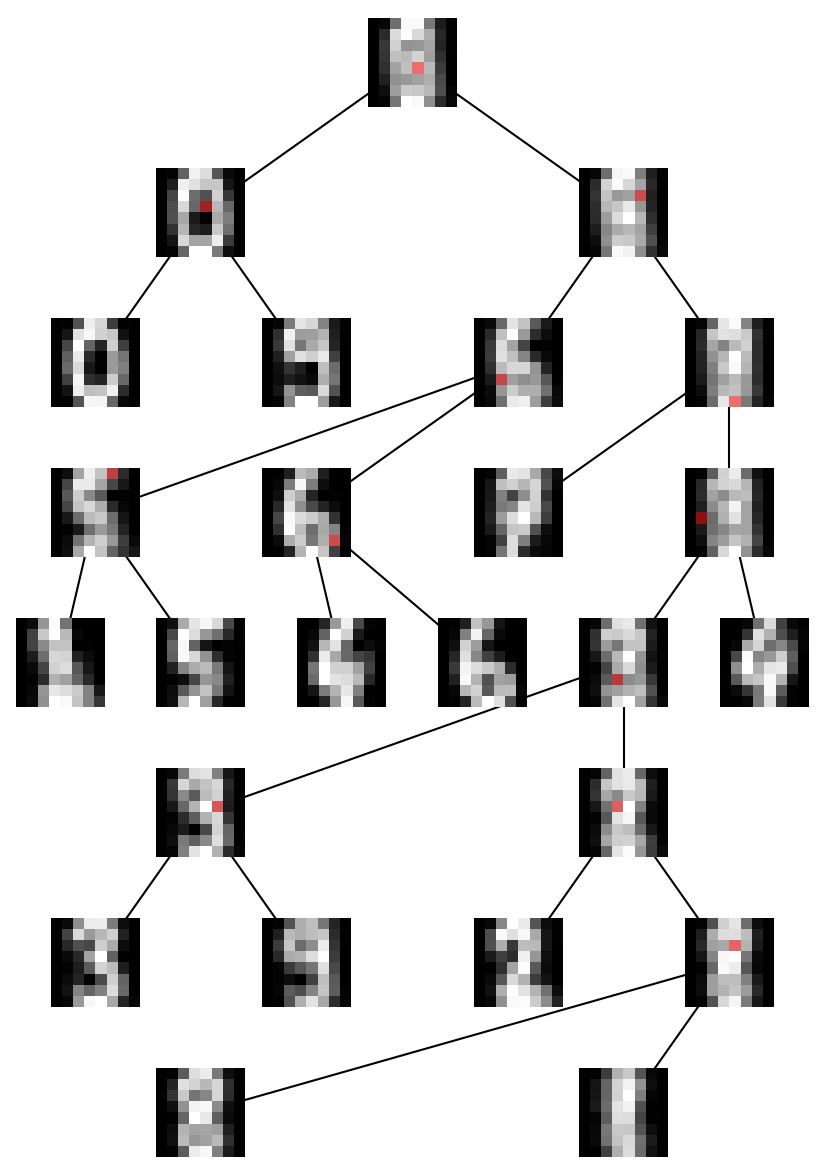
\includegraphics[width=\textwidth]{img/capN_interpretacion_arbol.png}\\
	\caption{Visualización de un árbol de clasificación para el dataset \textit{mnist}.}
\end{figure}

Usando las variables que se usaron para cortar cada nodo y los valores para el corte óptimo, podemos explicar la diferencia en estimaciones obtenidas. A esto lo llamamos capacidad de interpretación, y es importante a la hora de usar aprendizaje de máquinas para decisiones con repercusión en el mundo real.

En este caso se ha ajustado un árbol para clasificar imágenes de dígitos escritos a mano (dataset \textit{mnist}). Acá, cada variable corresponde a un pixel en particular, que en la figura están detacados en rojo. Cuando se llegan a hojas del árbol se logra, en muchos casos, distinguir dígitos. Por otro lado, nodos intermedios denotan conjuntos impuros (con varios dígitos posibles), de los cuales es necesario realizar un corte. Se visulumbran entonces que pixeles son más importantes a la hora de distinguir dígitos y que desencadenan en la decisión tomada por el árbol de clasificación.


\subsection{Bagging}
\label{sec:bagging}

\subsubsection{Método Bootstrapping}

\subsubsection{Bagging: agregación de modelos}

\subsubsection{Bosques aleatorios y variaciones}


\subsection{Boosting}
\label{sec:boosting}

\subsubsection{Motivación: algoritmos fuertes versos débiles}

\subsubsection{Algoritmo \textit{AdaBoost}}

\subsubsection{Modelamiento aditivo por etapas}

\subsubsection{\textit{GradientBoosting}: boosting como descenso de gradiente funcional}

\subsubsection{Más pérdidas y variaciones}
